%============================================================
% main.tex — IEEEtran split template (PW4 LUNA16 Detection)
%============================================================
\documentclass[conference]{IEEEtran}

% -------------------- Packages --------------------
\usepackage{graphicx}
\usepackage{float}
\usepackage{booktabs}
\usepackage{amsmath, amssymb}
\usepackage{siunitx}
\usepackage{hyperref}
\usepackage{xcolor}
\usepackage{subcaption}
\usepackage{cite}

\hypersetup{
  colorlinks=true,
  linkcolor=blue,
  urlcolor=blue,
  citecolor=blue
}

% Put your figures in /figure
\graphicspath{{figure/}}

\title{Pulmonary Nodule Detection in CT Scans\\
A Baseline Volumetric (3D) Detector on LUNA16}

\author{
\IEEEauthorblockN{Nugyen The Cuong}
\IEEEauthorblockN{22BA13058}
\IEEEauthorblockA{
Computed Tomography / Machine Learning in Medicine 2026\\
University of Science and Technology of Hanoi (USTH)\\
Email: cuongnt.22ba13058@usth.edu.vn
}
}

\setlength{\parindent}{0pt}
\setlength{\parskip}{1pt}

\begin{document}
\maketitle

\begin{abstract}
This report presents Practical Work 4: pulmonary nodule detection from CT scans using a small local subset of LUNA16. The task is volumetric (3D) detection, meaning the system must process a full CT volume and output 3D nodule locations with confidence scores.

We implement a simple baseline pipeline. First, we generate candidate points inside the lung region using basic image processing. Then, we use one deep learning model (a lightweight 3D CNN) to classify 3D patches around these candidates and reduce false positives. Besides detection-level evaluation, we also report patch-classification performance of the CNN. On a validation set at threshold 0.5, the classifier reaches 0.833 accuracy and an F1-score of 0.800, with recall of 1.000. We discuss typical errors and show how hyperparameters such as patch size and threshold affect results.
\end{abstract}

\section{Introduction}
Lung cancer screening CT contains a large number of slices and requires significant radiologist effort. Computer-aided detection (CAD) aims to automatically detect pulmonary nodules and reduce workload while improving sensitivity. This assignment requires building one machine learning/deep learning model capable of volumetric (3D) detection on an input CT volume.

In this work, we implement a baseline 3D detector following a common two-stage CAD design: (i) high-sensitivity candidate generation and (ii) false-positive reduction using a 3D CNN. LUNA16 provides standardized CT scans and reference nodule annotations to enable fair comparisons~\cite{setio2017luna16}. We evaluate our local subset and discuss differences between our baseline and top-performing systems reported on the public leaderboard.
\section{Dataset}
\subsection{LUNA16 overview}
LUNA16 (LUng Nodule Analysis 2016) is a curated subset of LIDC-IDRI designed for standardized lung nodule detection evaluation~\cite{setio2017luna16}. The full LUNA16 dataset contains 888 CT scans with slice thickness constrained to allow robust 3D analysis. Nodules in the reference standard are those with diameter $\geq 3$ mm that achieve majority agreement among expert annotators.

\subsection{Data format}
Each scan is provided in MetaImage format: a header file (\texttt{.mhd}) and voxel data file (\texttt{.raw}). The \texttt{.mhd} file stores metadata such as voxel dimensions, physical spacing (mm), origin, and (optionally) direction/transform matrix. The CT values are stored as 16-bit integers and typically correspond to Hounsfield Units (HU).

\subsection{Annotations}
We use \texttt{annotations.csv} from LUNA16 which provides:
\begin{itemize}
  \item \texttt{seriesuid}: unique scan identifier
  \item \texttt{coordX, coordY, coordZ}: nodule center in world coordinates (mm)
  \item \texttt{diameter\_mm}: nodule diameter in mm
\end{itemize}
To align annotations with the voxel grid, world coordinates are converted to voxel indices using image origin, spacing, and direction (we use SimpleITK physical-to-index transforms in code).

\subsection{Subset used in this practical work}
Due to compute limits, we trained and evaluated on a small subset of the full dataset that we downloaded locally. Table~\ref{tab:subset} summarizes our subset. 

\begin{table}[H]
\centering
\caption{Local LUNA16 subset used in this work (fill in).}
\label{tab:subset}
\begin{tabular}{lcc}
\toprule
Item & Count & Notes \\
\midrule
CT scans downloaded & \textbf{12} & From LUNA16 subsets \\
Annotated nodules in subset & \textbf{14} & From \texttt{annotations.csv} \\
Voxel spacing range (mm) & \textbf{0.488--2.500} & Before resampling \\
\bottomrule
\end{tabular}
\end{table}

\subsection{Preprocessing}
We clip HU values to $[-1000, 400]$ and normalize to $[0,1]$. Optionally, we resample scans to isotropic spacing (1.0 mm) to standardize patch geometry. A coarse lung mask is created using HU thresholding (HU $<-400$) and connected-component filtering.
\section{Methods}
\subsection{Problem formulation}
Given a CT volume, the goal is to output a set of detections
\[
\mathcal{D}=\{(x_i,y_i,z_i,s_i)\}_{i=1}^{M}
\]
where $(x_i,y_i,z_i)$ is the predicted nodule center in world coordinates (mm) and $s_i \in [0,1]$ is a confidence score.

\subsection{Pipeline overview}
We implement a two-stage baseline:
\begin{enumerate}
  \item \textbf{Candidate generation:} generate many suspicious 3D locations from the full volume with high sensitivity.
  \item \textbf{False-positive reduction (ONE deep model):} a 3D CNN classifies cubic patches centered at candidates as nodule / non-nodule.
\end{enumerate}
Although the system contains two stages, only \emph{one} learning model is used (the 3D CNN). Candidate generation is a deterministic image processing step.

\subsection{Candidate generation}
We generate candidates inside a coarse lung mask. Candidate points are obtained by applying a Laplacian-of-Gaussian (LoG) blob response (SciPy implementation) and non-maximum suppression to keep local maxima. We keep at most $K$ candidates per scan ($K=250$).

\subsection{3D CNN model}
We use a lightweight 3D CNN for binary classification of 3D patches of size $P\times P\times P$:
\begin{itemize}
  \item Conv3D(1$\rightarrow$16) + ReLU + MaxPool
  \item Conv3D(16$\rightarrow$32) + ReLU + MaxPool
  \item Conv3D(32$\rightarrow$64) + ReLU
  \item Global average pooling + Linear(64$\rightarrow$1)
\end{itemize}
The network outputs a logit, trained with BCEWithLogitsLoss. At inference, sigmoid converts logits to probabilities.

\subsection{Training data construction}
Positive samples are patches centered at annotated nodules; we apply small random jitter (few voxels) to increase robustness. Negative samples are patches sampled from lung regions away from annotated centers. Class imbalance is handled by sampling multiple negatives per positive and/or using \texttt{pos\_weight}.

\subsection{Inference and post-processing}
For each scan:
\begin{enumerate}
  \item Generate candidates $\{c_j\}_{j=1}^{K}$
  \item Extract patches and compute scores $s_j$
  \item Keep detections with $s_j \ge \tau$
  \item Merge close detections using greedy NMS in mm distance (e.g., 10 mm)
  \item Convert voxel indices back to world coordinates and export detections to CSV
\end{enumerate}

\subsection{Evaluation}
LUNA16 uses FROC analysis; the common summary score CPM is the average sensitivity at predefined false positive rates per scan: $\{0.125, 0.25, 0.5, 1, 2, 4, 8\}$~\cite{setio2017luna16}. In this practical work, we implement a simplified CPM approximation on our subset:
\begin{itemize}
  \item A detection is matched to a ground truth nodule if within a radius proportional to diameter (at least a small floor in mm).
  \item Unmatched detections count as false positives.
\end{itemize}.
\section{Results}
\subsection{Experimental setup}
Table~\ref{tab:trainsetup} lists our default training settings. (Fill with your actual values from the notebook/script.)

\begin{table}[H]
\centering
\caption{Training setup (fill in).}
\label{tab:trainsetup}
\begin{tabular}{lc}
\toprule
Parameter & Value \\
\midrule
Patch size $P$ & \textbf{48} \\
Resampling & \textbf{Yes} (target spacing: \textbf{1.0 mm isotropic}) \\
Candidates per scan $K$ & \textbf{400} \\
Batch size & \textbf{8} \\
Epochs & \textbf{8} \\
Optimizer & Adam ($\text{lr}=\textbf{1e-3}$) \\
Threshold $\tau$ & \textbf{0.5} \\
NMS distance & \textbf{10.0 mm} \\
\bottomrule
\end{tabular}
\end{table}

\subsection{Patch classification metrics (false-positive reduction model)}
To better understand the quality of the 3D CNN classifier used in our detection pipeline, we evaluate it as a binary patch classifier. We use a decision threshold of 0.5 (sigmoid probability). The validation set contains 12 patches in total.

Table~\ref{tab:cls_metrics} reports standard classification metrics. The results show that the model achieves perfect recall (no missed positive patches), but the precision is lower because there is still one false positive. This behavior is often acceptable in detection because missing nodules is usually more serious than producing a small number of additional candidates.

\begin{table}[H]
\centering
\caption{Patch classification performance at threshold 0.5 (validation).}
\label{tab:cls_metrics}
\begin{tabular}{lc}
\toprule
Metric & Value \\
\midrule
Accuracy & 0.8333 \\
Precision & 0.6667 \\
Recall (Sensitivity) & 1.0000 \\
F1-score & 0.8000 \\
Specificity & 0.7500 \\
\bottomrule
\end{tabular}
\end{table}

\begin{table}[H]
\centering
\caption{Confusion matrix at threshold 0.5 (validation patches).}
\label{tab:confusion}
\begin{tabular}{lcc}
\toprule
 & Pred 0 & Pred 1 \\
\midrule
True 0 & 7 & 1 \\
True 1 & 0 & 4 \\
\bottomrule
\end{tabular}
\end{table}

\begin{figure}[H]
\centering
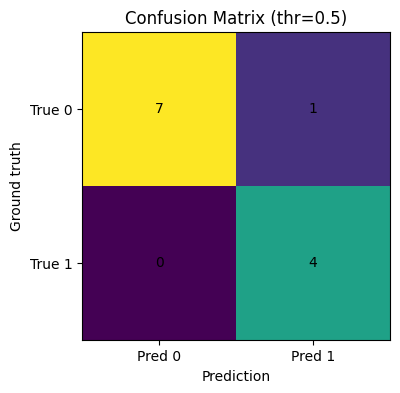
\includegraphics[width=0.70\linewidth]{confusion_matrix_thr05.png}
\caption{Confusion matrix of the patch classifier at threshold 0.5.}
\label{fig:cm}
\end{figure}

\noindent\textbf{} 

Figure~\ref{fig:train_curve} shows the training and validation loss over 8 epochs using \texttt{BCEWithLogitsLoss}. Overall, both curves go down, which means the 3D CNN learns useful patterns from the patches. The validation loss decreases strongly at the last epoch and ends below the training loss, suggesting that the model generalizes reasonably well on this split. We also observe a small instability around epochs 5--6 where the validation loss increases while the training loss continues to decrease. This behaviour is common when the validation set is small or when the model starts to fit specific training samples. In practice, this indicates that early stopping or stronger regularization (more negative samples, augmentation, or weight decay) could make training more stable.

\begin{figure}[H]
\centering
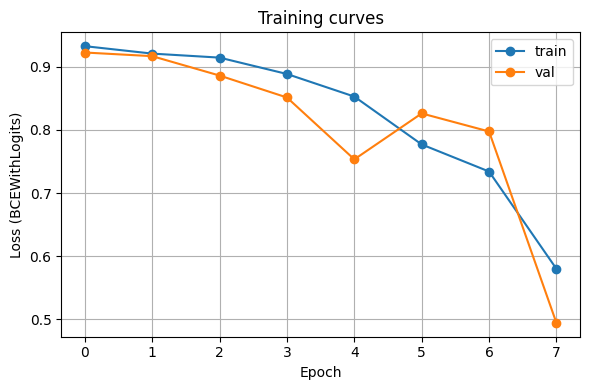
\includegraphics[width=0.70\linewidth]{training_curve.png}
\caption{Training and validation loss over 8 epochs using BCEWithLogitsLoss.}
\label{fig:train_curve}
\end{figure}
\section{Discussion}
\subsection{Why our baseline is weaker than the leaderboard}
Our results are expected to be below leaderboard performance due to:
\begin{itemize}
  \item \textbf{Small subset training:} fewer scans reduces generalization.
  \item \textbf{Simplified candidate generation:} LoG peak detection may miss complex nodules or generate many false positives.
  \item \textbf{Lightweight 3D CNN:} limited capacity compared to modern multi-scale 3D architectures.
  \item \textbf{Approximate evaluation:} our simplified CPM differs from official LUNA16 scoring rules.
\end{itemize}

\subsection{Failure cases}
Common errors we observed:
\begin{itemize}
  \item \textbf{False positives} near vessels, airway walls, or pleura (high-contrast structures).
  \item \textbf{Missed small nodules} when candidate generation fails (low-contrast regions).
  \item \textbf{Close detections} merged incorrectly if NMS distance is too large.
\end{itemize}

\subsection{Effect of hyperparameters}
Patch size affects context: larger patches capture more anatomy but may dilute signal; threshold $\tau$ trades off FP/scan and sensitivity. Candidate limit $K$ influences runtime and maximum sensitivity.

\subsection{Interpretation of classification metrics}
On the validation set, the patch classifier achieves recall of 1.000 and F1-score of 0.800 at threshold 0.5. This means the model did not miss any positive patch in this split. However, precision is 0.6667 because one negative patch is predicted as positive. In the detection pipeline, this type of error increases false positives, so more post-processing or stronger negative sampling (hard negatives near vessels) could improve precision.
\section{Conclusion and future work}
We implemented a complete volumetric (3D) pulmonary nodule detection pipeline on LUNA16 CT scans using a single learning model (3D CNN) for false-positive reduction. The system processes full volumes, generates candidates, predicts confidence scores, and exports 3D detections.

Future improvements include:
\begin{itemize}
  \item More robust candidate generation (multi-scale, learned proposals)
  \item Stronger 3D backbones (ResNet-style blocks, multi-scale feature extraction)
  \item Hard negative mining to reduce vessel-related false positives
  \item Training on the full 888-scan LUNA16 set with official evaluation code
\end{itemize}

\begin{thebibliography}{9}

\bibitem{setio2017luna16}
A. A. A. Setio et al.,
``Validation, comparison, and combination of algorithms for automatic detection of pulmonary nodules in computed tomography images: The LUNA16 challenge,''
\emph{Medical Image Analysis}, 2017.

\bibitem{luna16site}
LUNA16 Grand Challenge website,
\emph{https://luna16.grand-challenge.org/}.

\bibitem{lidc}
S. G. Armato III et al.,
``The Lung Image Database Consortium (LIDC) and Image Database Resource Initiative (IDRI): A completed reference database of lung nodules on CT scans,''
\emph{Medical Physics}, 2011.

\end{thebibliography}

\end{document}